\documentclass[../../main]{subfiles}

\renewcommand\thesection{\arabic{section}}


\begin{document}

\section{Bread and Butter of TinyML Workflow} \label{sec:}

As we can see from figure \ref{fig:designFlowTinyML}, the core part of the
workflow is the \emph{compression techniques} we use. Let's see an overview
of each of these techniques.

\subsection{Quantization}

One way to shrink the model size is \emph{quantize} the coefficients in our
question matrix. The coefficients usually will be $32$ bit integers.
We need to map them into $8$ bit integers. This process is know as
\emph{Quantization}.

\begin{figure} [H]
    \centering
    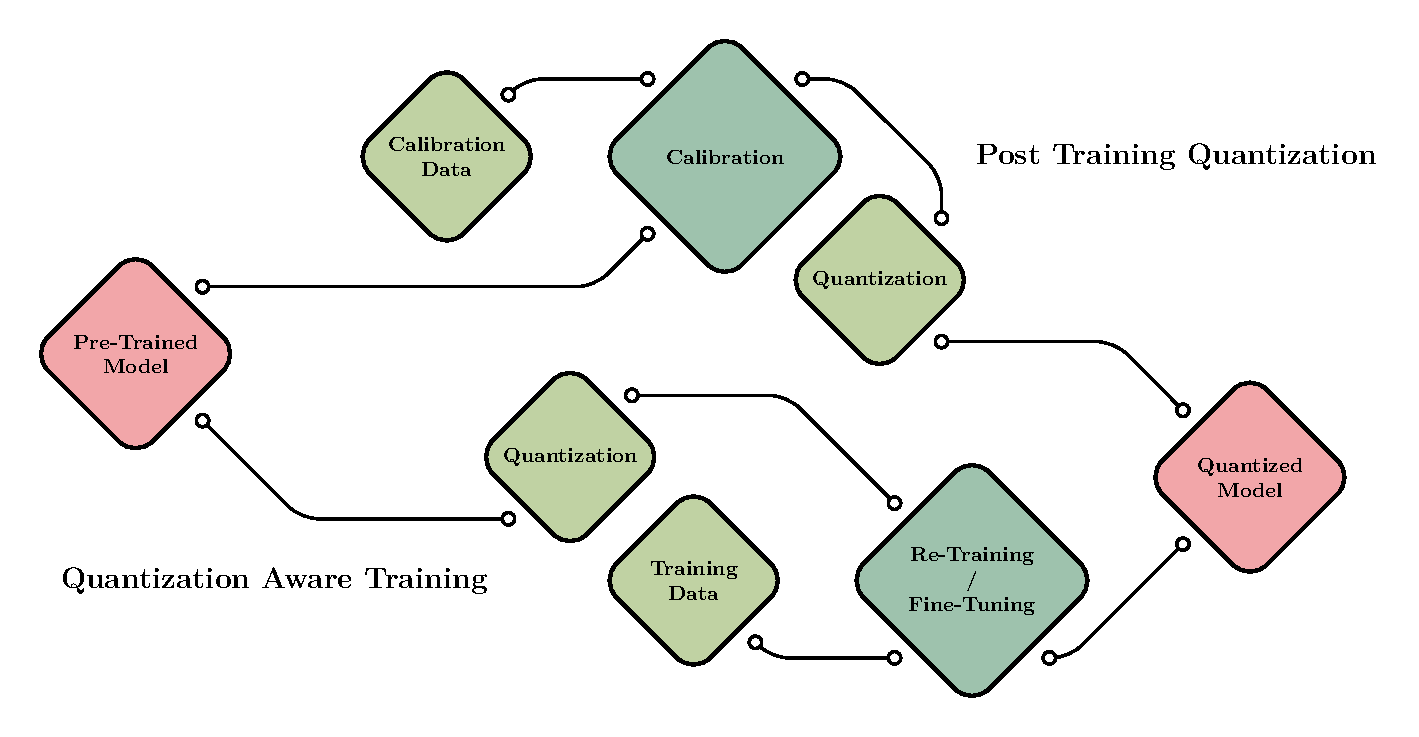
\includegraphics [
        max width = \IGXMaxWidth,
        max height = \IGXMaxHeight,
        \IGXDefaultOptionalArgs,
    ] {pics/endQuantization.pdf}
    \captionof{figure} {Two different ways to do Quantization.}
    \label{fig:quantizationTinyML}
\end{figure}

Figure \ref{fig:quantizationTinyML} show two ways to quantize our trained model. One
is \emph{Quantization Aware Training} and the other is \emph{Post Training Quantization}.

\begin{itemize}
    \item \textsc{Quantization Aware Training:}
        \begin{itemize} [label=]
            \item If we have enough data, we can leverage it to tweak and tune the
                model after the quantization process. What we are doing is essentially
                re-training the model once more after the quantization. Therefore the
                name Quantization Aware Training. See figure \ref{fig:quantizationTinyML}
                to get a better idea.
        \end{itemize}

    \item \textsc{Post Training Quantization:}
        \begin{itemize} [label=]
            \item In Post Training Quantization, we are simply quantizing after an
                initial calibration process. Even though this gets the job done, it
                is preferable to do QAT when ever possible.
        \end{itemize}

\end{itemize}

\subsection{Pruning}

We can think of our ML model as a bunch of neurons connected to each other through
different connections. As shown in figure \ref{fig:pruningTinyML}, we can think of
them having different layers, carrying out different tasks or looking for certain
features in the data. But not all of these connections will have a significant
influence in next layer. So we can cut these less influencing connection and
still keep the performance almost the same. This process is know as \emph{pruning}.

% From figure \ref{fig:pruningTinyML}

\begin{figure} [H]
    \centering
    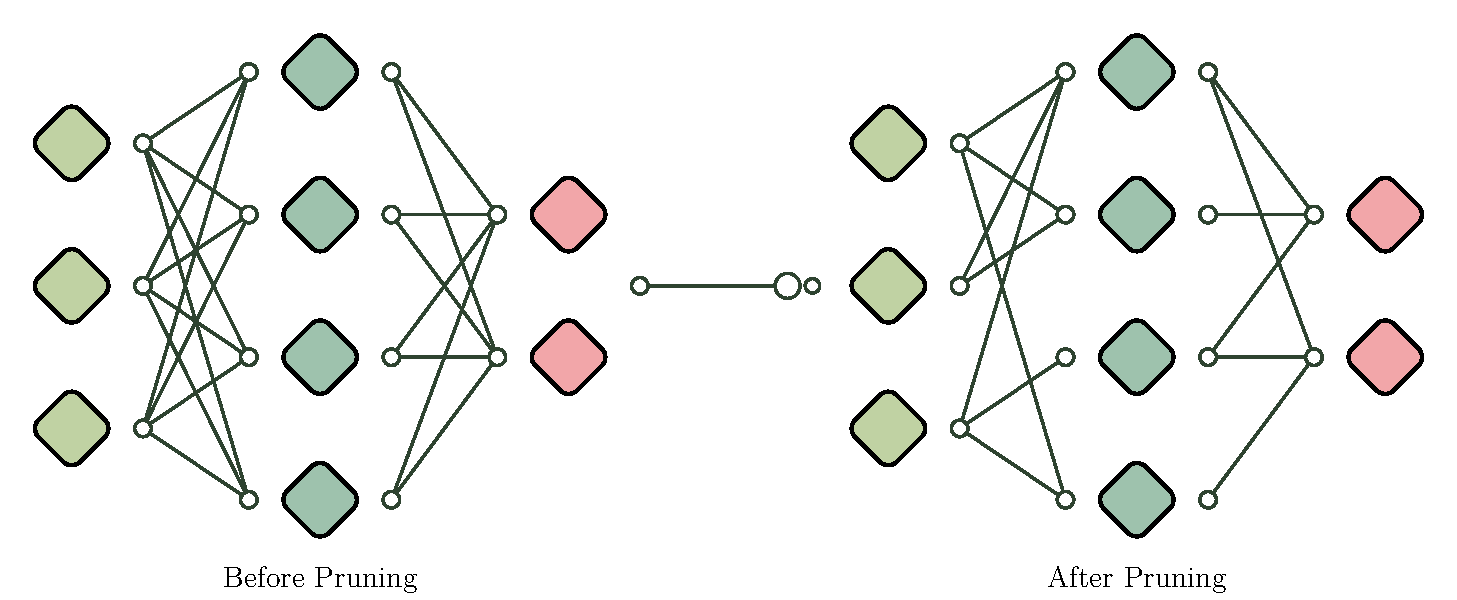
\includegraphics [
        max width = 0.9\textwidth,
        max height = \IGXMaxHeight,
        \IGXDefaultOptionalArgs,
    ] {pics/endPruning.pdf}
    \captionof{figure} {Pruning process in TinyML.}
    \label{fig:pruningTinyML}
\end{figure}

What we are essentially doing is zeroing out some of the coefficients in the
question matrix that represents the connections. In short, we are generating a
more \emph{sparse} question matrix. And we can store these sparse matrices
in a more compact way. Thereby decreasing the size of the model.

\subsection{Knowledge Distillation}

In this technique, we will train two models. One is know as the \emph{teacher model}
and the other is know as the \emph{student model}. At first we will train the teacher
model, then we will use this teacher model to \emph{soft label} the data. Then we
will use the hard and soft labelled data to train the student model.

\begin{figure} [H]
    \centering
    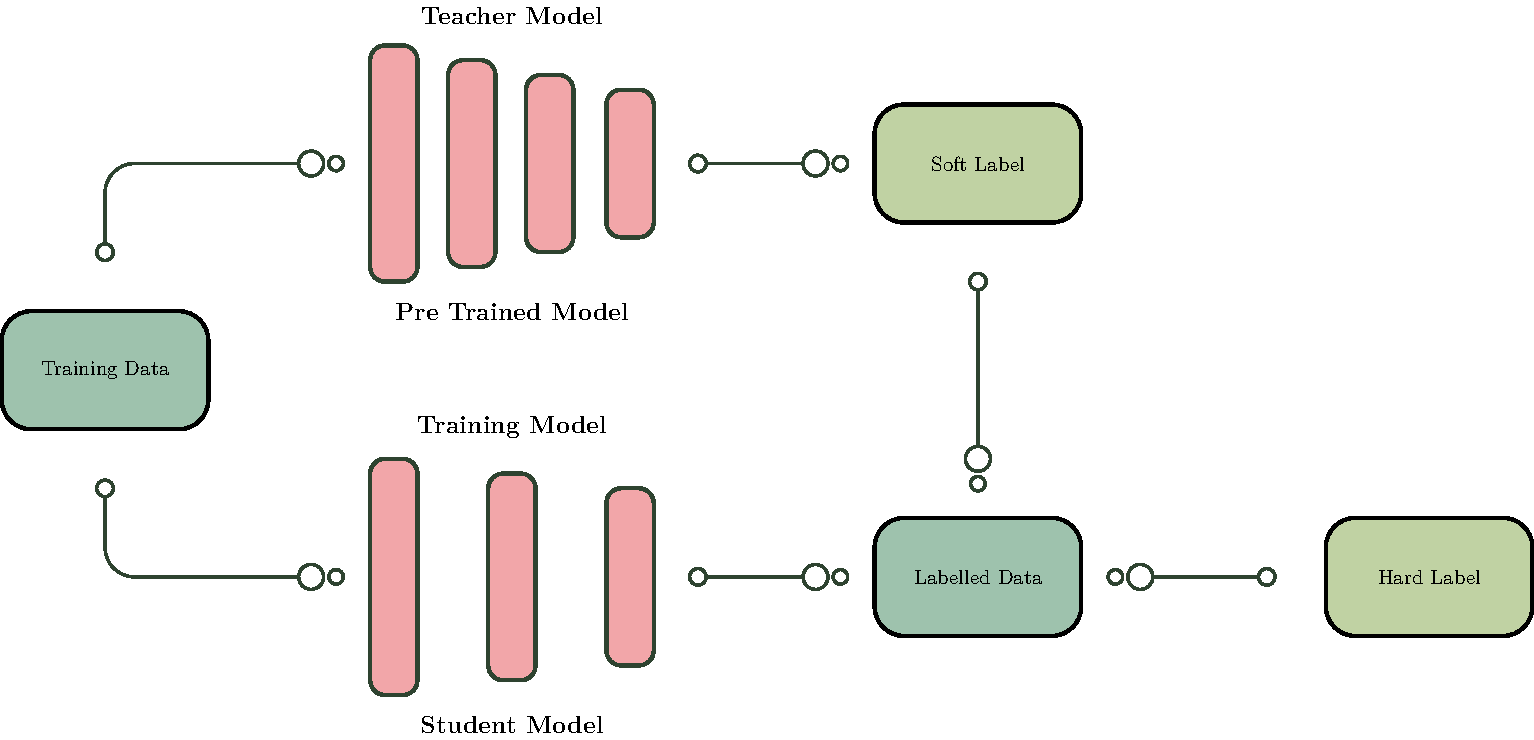
\includegraphics [
        max width = \IGXMaxWidth,
        max height = \IGXMaxHeight,
        \IGXDefaultOptionalArgs,
    ] {pics/endKnowledgeDistillation.pdf}
    \captionof{figure} {Technique of knowledge distillation in TinyML.}
    \label{fig:knowledgeTinyML}
\end{figure}

Figure \ref{fig:knowledgeTinyML} shows the exact process. This additional help
from the teacher model helps the student model to fit to the data quicker.
The student model will be much more performant with negligible decrease in
accuracy than the teacher model.

\end{document}
